% Options for packages loaded elsewhere
\PassOptionsToPackage{unicode}{hyperref}
\PassOptionsToPackage{hyphens}{url}
%
\documentclass[
]{article}
\usepackage{lmodern}
\usepackage{amssymb,amsmath}
\usepackage{ifxetex,ifluatex}
\ifnum 0\ifxetex 1\fi\ifluatex 1\fi=0 % if pdftex
  \usepackage[T1]{fontenc}
  \usepackage[utf8]{inputenc}
  \usepackage{textcomp} % provide euro and other symbols
\else % if luatex or xetex
  \usepackage{unicode-math}
  \defaultfontfeatures{Scale=MatchLowercase}
  \defaultfontfeatures[\rmfamily]{Ligatures=TeX,Scale=1}
\fi
% Use upquote if available, for straight quotes in verbatim environments
\IfFileExists{upquote.sty}{\usepackage{upquote}}{}
\IfFileExists{microtype.sty}{% use microtype if available
  \usepackage[]{microtype}
  \UseMicrotypeSet[protrusion]{basicmath} % disable protrusion for tt fonts
}{}
\makeatletter
\@ifundefined{KOMAClassName}{% if non-KOMA class
  \IfFileExists{parskip.sty}{%
    \usepackage{parskip}
  }{% else
    \setlength{\parindent}{0pt}
    \setlength{\parskip}{6pt plus 2pt minus 1pt}}
}{% if KOMA class
  \KOMAoptions{parskip=half}}
\makeatother
\usepackage{xcolor}
\IfFileExists{xurl.sty}{\usepackage{xurl}}{} % add URL line breaks if available
\IfFileExists{bookmark.sty}{\usepackage{bookmark}}{\usepackage{hyperref}}
\hypersetup{
  hidelinks,
  pdfcreator={LaTeX via pandoc}}
\urlstyle{same} % disable monospaced font for URLs
\usepackage[margin=1in]{geometry}
\usepackage{graphicx}
\makeatletter
\def\maxwidth{\ifdim\Gin@nat@width>\linewidth\linewidth\else\Gin@nat@width\fi}
\def\maxheight{\ifdim\Gin@nat@height>\textheight\textheight\else\Gin@nat@height\fi}
\makeatother
% Scale images if necessary, so that they will not overflow the page
% margins by default, and it is still possible to overwrite the defaults
% using explicit options in \includegraphics[width, height, ...]{}
\setkeys{Gin}{width=\maxwidth,height=\maxheight,keepaspectratio}
% Set default figure placement to htbp
\makeatletter
\def\fps@figure{htbp}
\makeatother
\setlength{\emergencystretch}{3em} % prevent overfull lines
\providecommand{\tightlist}{%
  \setlength{\itemsep}{0pt}\setlength{\parskip}{0pt}}
\setcounter{secnumdepth}{-\maxdimen} % remove section numbering
\usepackage{ctex}
\usepackage{xcolor}
\usepackage{fancyhdr}
\pagestyle{fancy}
\cfoot{\thepage}
\usepackage{sectsty}
\definecolor{glaucous}{rgb}{0.38, 0.51, 0.71}
\definecolor{lavenderblush}{rgb}{1.0, 0.94, 0.96}
\usepackage{enumitem}% http://ctan.org/pkg/enumitem
\usepackage[empty]{fullpage}% http://ctan.org/pkg/fullpage
\usepackage{color}% http://ctan.org/pkg/color
\usepackage{hyperref}% http://ctan.org/pkg/hyperref
\usepackage{geometry}
\geometry{a4paper,scale=1}
\usepackage{blindtext}
\usepackage[center]{caption}
\usepackage{subfigure}
\usepackage{float}
\usepackage{graphicx}
\usepackage{booktabs}
\usepackage[justification=centering]{caption}
\usepackage{threeparttable}
\usepackage{longtable}
\usepackage{array}
\usepackage{multirow}
\usepackage{wrapfig}
\usepackage{float}
\usepackage{colortbl}
\usepackage{pdflscape}
\usepackage{tabu}
\usepackage{threeparttable}
\usepackage{threeparttablex}
\usepackage[normalem]{ulem}
\usepackage{makecell}
\usepackage{xcolor}
\linespread{1.0}
\setlength{\parskip}{0.5em}
\setlength{\footskip}{20pt}
\linespread{1.15}
\setlength{\parskip}{0.3em}
\textwidth 7in
\textheight 9.95in
\oddsidemargin -.25in
\evensidemargin -.25in
\topmargin -1in
\usepackage{booktabs}
\usepackage{longtable}
\usepackage{array}
\usepackage{multirow}
\usepackage{wrapfig}
\usepackage{float}
\usepackage{colortbl}
\usepackage{pdflscape}
\usepackage{tabu}
\usepackage{threeparttable}
\usepackage{threeparttablex}
\usepackage[normalem]{ulem}
\usepackage{makecell}
\usepackage{xcolor}

\title{\textcolor{glaucous}{\Huge \textbf {新冠早报}}}
\usepackage{etoolbox}
\makeatletter
\providecommand{\subtitle}[1]{% add subtitle to \maketitle
  \apptocmd{\@title}{\par {\large #1 \par}}{}{}
}
\makeatother
\subtitle{\textcolor{glaucous}{\Large 第六期 3月28日}}
\author{}
\date{\vspace{-2.5em}}

\begin{document}
\maketitle

\fontsize{13}{13}
\selectfont
\vspace{-10truemm}

\newcommand{\resheading}[1]{%
  \noindent\fcolorbox{lavenderblush}{lavenderblush}{\makebox[\dimexpr\textwidth-2\fboxsep-2\fboxrule][l]{\textbf{~#1}}}%
}

\pagestyle{fancyplain}
\lhead{
\includegraphics[height=2cm]{./input/logo.png}}
\rhead{
\begin{tabular}{ccc}
\textcolor{gray}{中美健康峰会「智援组」新冠早报组}\\
\\ \\ \\ \\ \\
\end{tabular}}

\renewcommand{\headrulewidth}{0pt}
\setlength{\headheight}{25pt}

%
  \noindent\fcolorbox{lavenderblush}{lavenderblush}{\makebox[\dimexpr\textwidth-2\fboxsep-2\fboxrule][l]{\textbf{~\Large 每日新闻}}}%

\hypertarget{section}{%
\subsection{\texorpdfstring{\textcolor{glaucous}{\Large 国际}}{}}\label{section}}

\textbf{\textcolor{glaucous}{英国广播公司(BBC)}}:
\textbf{世界银行宣布19亿美元紧急资金}

据4月2日的报道称,世界银行已启动了一项19亿美元的应急基金,以帮助25个国家应
对新冠病毒大流行。 其中,印度将获得最大的一笔资金(10亿美元)来改善新冠筛
查、追踪和实验室诊断,资金还将用于购买个人防护设备和建立隔离病房。

\textbf{\textcolor{glaucous}{有线电视新闻网(CNN)}} :
\textbf{120万个N95口罩正从中国运往美国}

当地时间4月1日,新英格兰爱国者队的飞机从中国深圳出发,运载120万个N95口罩前
往美国,预计将于4月2日达到波士顿洛根机场。

\textbf{\textcolor{glaucous}{有线电视新闻网(CNN)}} :
\textbf{美国总统特朗普启用国防生产法,点名七家公司生产呼吸机}

当地时间4月2日,白宫发布声明称,美国总统特朗普下令全面启用国防生产法,并在
声明中点名希望通用电气、美敦力、飞利浦等七家美国公司可以通过此法案更顺利地
获取生产呼吸机所需的材料。

\textbf{\textcolor{glaucous}{环球时报(Global Times)}} :
\textbf{意大利医护人员感染超1万}

当地时间4月2日,意大利外科和牙科医生联合会发布公告称,意大利自疫情爆发以来
因感染新冠肺炎去世的医生达69人;另据卫生医疗行业协会通报,意大利目前感染新
冠肺炎的医护人员超过1万例。

\textbf{\textcolor{glaucous}{有线电视新闻网(CNN)}} :
\textbf{澳大利亚将有100万家庭获得免费托儿服务}

当地时间4月2日,澳大利亚总理斯科特·莫里森宣布,由于新冠肺炎疫情影响,澳大
利亚计划为约100万个家庭提供免费托儿服务。

\textbf{\textcolor{glaucous}{非洲疾控中心(Africa CDC)}} :
\textbf{非洲新冠肺炎超7000例 蔓延50国}

截至非洲东部时间4月3日17时,非洲共有50国出现新冠肺炎疫情,总数达7123例,死
亡289例,治愈592例。

\hypertarget{section-1}{%
\subsection{\texorpdfstring{\textcolor{glaucous}{\Large 国内}}{}}\label{section-1}}

\textbf{\textcolor{glaucous}{财新网(Caixin.com)}}:
\textbf{李文亮江学庆等14人获评烈士}

北京时间4月2日,湖北省人民政府评定王兵、冯效林、江学庆、刘智明、李文亮、张
抗美、肖俊、吴涌、柳帆、夏思思、黄文军、梅仲明、彭银华、廖建军等14名牺牲在
新冠肺炎疫情防控一线人员为首批烈士。

\textbf{\textcolor{glaucous}{中国日报(China Daily)}}:
\textbf{中国安排9次包机从海外接回1457人}

北京时间4月2日,外交部副部长马兆旭表示,中国在3月安排了9次包机,将1457名海
外的中国公民带回国,其中包括来自伊朗,意大利等国家的海外留学生。

\newpage

%
  \noindent\fcolorbox{lavenderblush}{lavenderblush}{\makebox[\dimexpr\textwidth-2\fboxsep-2\fboxrule][l]{\textbf{~\Large 疫情观察}}}%

\begin{small}
{数据源:约翰霍普金斯大学,The COVID Tracking Project \quad   数据截止至:北京时间3月28日 早4:00}
\end{small}

\hypertarget{section-2}{%
\section{\texorpdfstring{\textcolor{glaucous}{一、世界疫情}}{}}\label{section-2}}

~~截止北京时间4月3日早5:00,全球累计确诊病例超过100万人(1,075,777),累计死亡52,772例。由图1所示,确诊病例全球分布广泛,主要集中在美国、亚洲、欧洲以及中东地区,在南美、澳大利亚以及非洲部分地区也有散在分布。由表1所示,累计确诊人数前三位的国家仍然为美国,意大利和西班牙。德国首次超过中国成为第四位。粗发病率最高的国家是西班牙和瑞士,均在200/10万人以上。此外,澳大利亚、加拿大累计确诊数均已超过1万人。

~~XXXXXXX。

\begin{figure}[H]
\caption{世界疫情分布图 (Global Map of Cumulative Confirmed COVID-19 Cases)} %最终文档中希望显示的图片标题
\centering
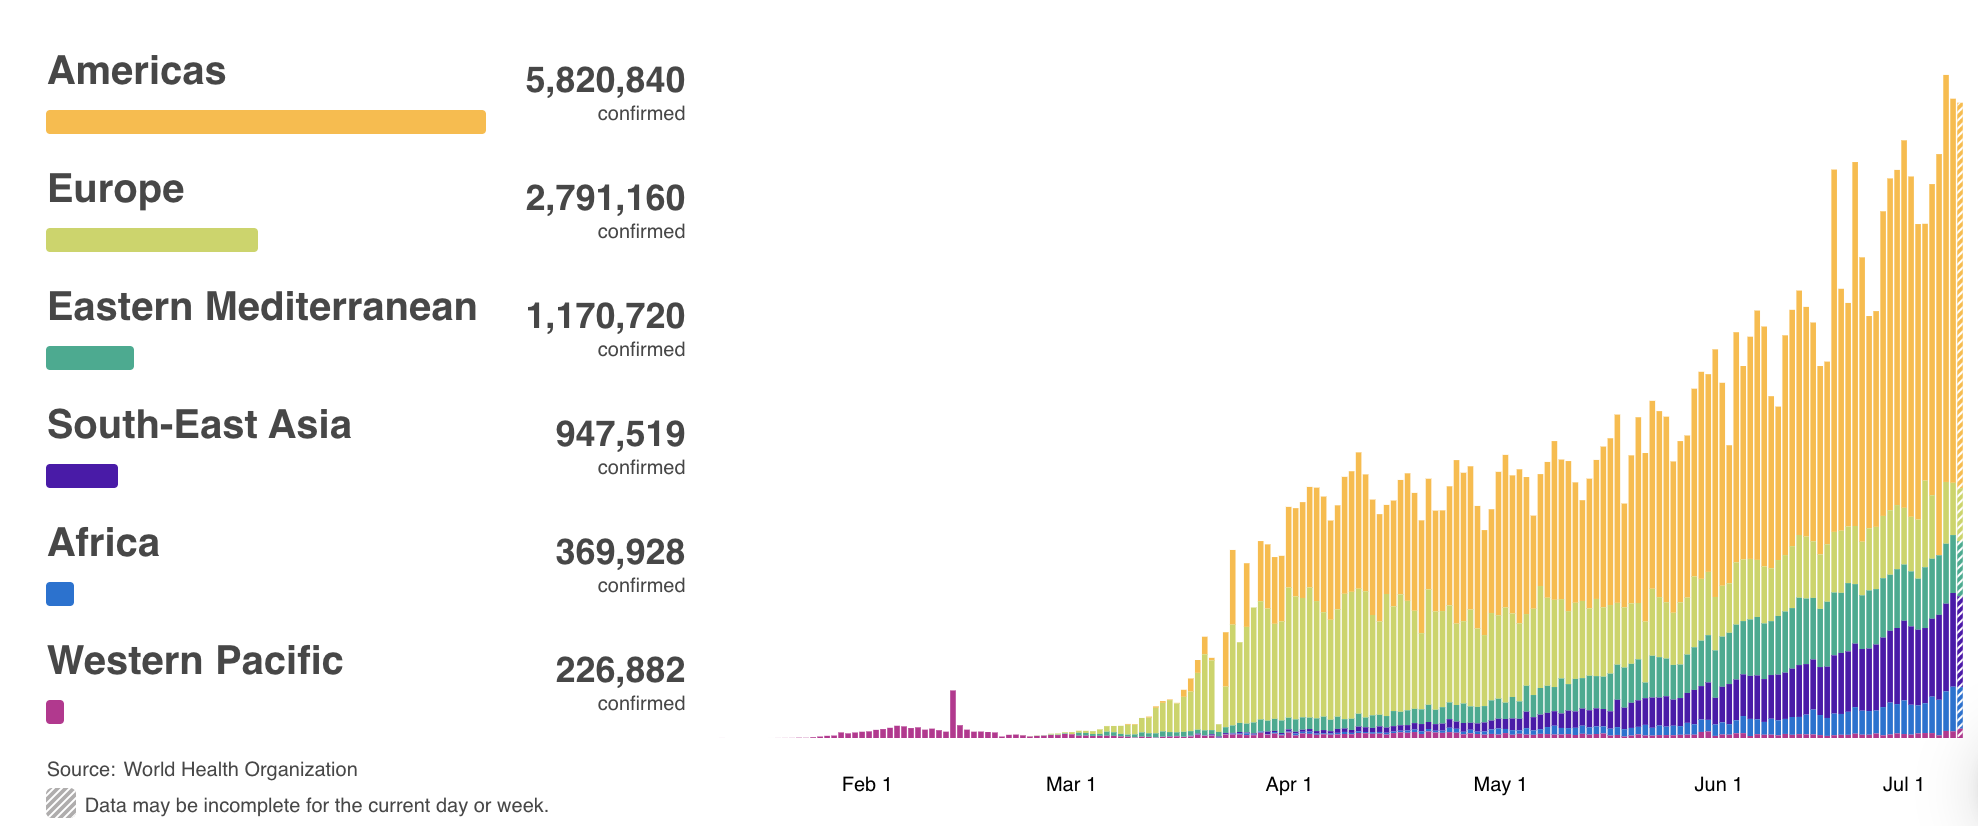
\includegraphics[]{./input/covid1.png} %插入图片,[]中设置图片大小,{}中是图片文件名
\label{} %用于文内引用的标签
\end{figure}

\begin{table}[H]
    \caption{<U+7D2F><U+8BA1><U+786E><U+8BCA><U+524D><U+5341><U+4F4D><U+56FD><U+5BB6>}
      \vspace{-0.5\baselineskip}
      \centering \begin{table}[H]
\centering
\begin{tabular}{rlrrr}
\toprule
  & <U+56FD><U+5BB6>(<U+5730><U+533A>) & <U+7D2F><U+8BA1><U+786E><U+8BCA><U+75C5><U+4F8B> & <U+603B><U+4EBA><U+53E3> & <U+7C97><U+53D1><U+75C5><U+7387>\\
\midrule
\rowcolor{gray!6}  1 & <U+7F8E><U+56FD> US & 368,241 & 331,002,651 & 111\\
2 & <U+897F><U+73ED><U+7259> Spain & 136,675 & 46,754,778 & 292\\
\rowcolor{gray!6}  3 & <U+610F><U+5927><U+5229> Italy & 132,547 & 60,461,826 & 219\\
4 & <U+5FB7><U+56FD> Germany & 103,375 & 83,783,942 & 123\\
\rowcolor{gray!6}  5 & <U+6CD5><U+56FD> France & 98,984 & 65,273,511 & 152\\
6 & <U+4E2D><U+56FD> China & 82,697 & 1,439,323,776 & 6\\
\rowcolor{gray!6}   & <U+6E56><U+5317> Hubei & 67,803 & 59,172,000 & 115\\
7 & <U+4F0A><U+6717> Iran & 60,500 & 83,992,949 & 72\\
\rowcolor{gray!6}  8 & <U+82F1><U+56FD> United Kingdom & 52,279 & 67,886,011 & 77\\
9 & <U+571F><U+8033><U+5176> Turkey & 30,217 & 84,339,067 & 36\\
\rowcolor{gray!6}  10 & <U+745E><U+58EB> Switzerland & 21,657 & 8,654,622 & 250\\
\bottomrule
\end{tabular}
\end{table} \begin{tablenotes}
        \footnotesize
        \item <U+6CE8>:<U+7C97><U+53D1><U+75C5><U+7387><U+5B9A><U+4E49>:<U+7D2F><U+8BA1><U+786E><U+8BCA><U+75C5><U+4F8B>/10<U+4E07><U+4EBA><U+3002><U+8BA1><U+7B97><U+65B9><U+5F0F>:(<U+7D2F><U+8BA1><U+786E><U+8BCA><U+75C5><U+4F8B>/<U+2F08>)×10<U+4E07>  %<U+6B64><U+5904><U+52A0><U+5165><U+6CE8><U+91CA><U+4FE1><U+606F>
      \end{tablenotes}
    \end{table}

\newpage

~~从表2和图2来看,美国新增病例数居全球首位,连续三天每日新增病例数稳定在约两万五千人。德国新增病例数近三日有小幅升高的趋势。法国新增病例数于3月31日达到近期峰值(7,657),近两日每日减少约2500人,疫情有趋稳的迹象。加拿大新增病例数进入前十位。此外,南美洲的巴西近三日新增病例数达到千人以上,南亚的印度新增病例数由3月31号之前的200人以下升高至500人以上。

~~从累计死亡病例数(表3和图3)来看,多数国家新增死亡病例数及病死率稳定。法国新增死亡病例数较昨日(+511人)升高幅度明显增加,病死率由7\%升高到9\%。美国和西班牙新增死亡数较昨日升高约300人,但病死率升高幅度不大(+0.3\%)。

\begin{table}
    \begin{minipage}{.4\linewidth}
    \centering
    \captionsetup{justification=centering}
    \caption{<U+65E5><U+65B0><U+589E><U+786E><U+8BCA><U+75C5><U+4F8B><U+56FD><U+5BB6><U+8D8B><U+52BF><U+56FE> \newline(<U+4E2D><U+56FD><U+53CA><U+5176><U+4ED6><U+524D><U+4E94><U+4F4D><U+56FD><U+5BB6>)}
    \vspace{-0.5\baselineskip}
      \centering
    \captionsetup{justification=centering} \begin{table}[H]
\centering
\begin{tabular}{rlr}
\toprule
  & <U+56FD><U+5BB6> & <U+5F53><U+65E5><U+65B0><U+589E><U+75C5><U+4F8B>\\
\midrule
\rowcolor{gray!6}  1 & <U+7F8E><U+56FD> US & 1,627\\
2 & <U+58A8><U+897F><U+54E5> Mexico & 296\\
\rowcolor{gray!6}  3 & <U+65E5><U+672C> Japan & 252\\
4 & <U+5DF4><U+62FF><U+9A6C> Panama & 112\\
\rowcolor{gray!6}  5 & <U+52A0><U+62FF><U+5927> Canada & 104\\
6 & <U+963F><U+6839><U+5EF7> Argentina & 74\\
\rowcolor{gray!6}  7 & <U+52A0><U+7EB3> Ghana & 73\\
8 & <U+5DF4><U+897F> Brazil & 71\\
\rowcolor{gray!6}  9 & <U+65B0><U+897F><U+5170> New Zealand & 54\\
10 & <U+97E9><U+56FD> Korea, South & 47\\
\bottomrule
\end{tabular}
\end{table} \end{minipage}%
    \begin{minipage}{.4\linewidth}
    \centering
    \captionsetup{justification=centering}
     \caption{<U+7D2F><U+8BA1><U+6B7B><U+4EA1><U+75C5><U+4F8B><U+56FD><U+5BB6><U+8D8B><U+52BF><U+56FE> \newline(<U+4E2D><U+56FD><U+53CA><U+5176><U+4ED6><U+524D><U+4E94><U+4F4D><U+56FD><U+5BB6>)}
     \vspace{-0.5\baselineskip}
      \centering
    \captionsetup{justification=centering} \begin{table}[H]
\centering
\begin{tabular}{rlrrr}
\toprule
  & <U+56FD><U+5BB6> & <U+7D2F><U+8BA1><U+6B7B><U+4EA1><U+75C5><U+4F8B> & <U+8F83><U+6628><U+65E5> & <U+75C5><U+6B7B><U+7387>\\
\midrule
\rowcolor{gray!6}  1 & <U+610F><U+5927><U+5229> Italy & 16,523 & 0 & 12.5\\
2 & <U+897F><U+73ED><U+7259> Spain & 13,341 & 0 & 9.8\\
\rowcolor{gray!6}  3 & <U+7F8E><U+56FD> US & 10,986 & 203 & 3.0\\
4 & <U+6CD5><U+56FD> France & 8,926 & 0 & 9.0\\
\rowcolor{gray!6}  5 & <U+82F1><U+56FD> United Kingdom & 5,385 & 0 & 10.3\\
6 & <U+4F0A><U+6717> Iran & 3,739 & 0 & 6.2\\
\rowcolor{gray!6}  7 & <U+4E2D><U+56FD> China & 3,335 & 0 & 4.0\\
8 & <U+8377><U+5170> Netherlands & 1,874 & 0 & 9.9\\
\rowcolor{gray!6}  9 & <U+5FB7><U+56FD> Germany & 1,810 & 0 & 1.8\\
10 & <U+6BD4><U+5229><U+6642> Belgium & 1,632 & 0 & 7.8\\
\bottomrule
\end{tabular}
\end{table} \end{minipage} 
\end{table}

\begin{figure}[H]
\centering
\begin{minipage}[b]{0.45\linewidth}
\caption{日新增确诊病例国家趋势图\\(中国及其他前五位国家)}
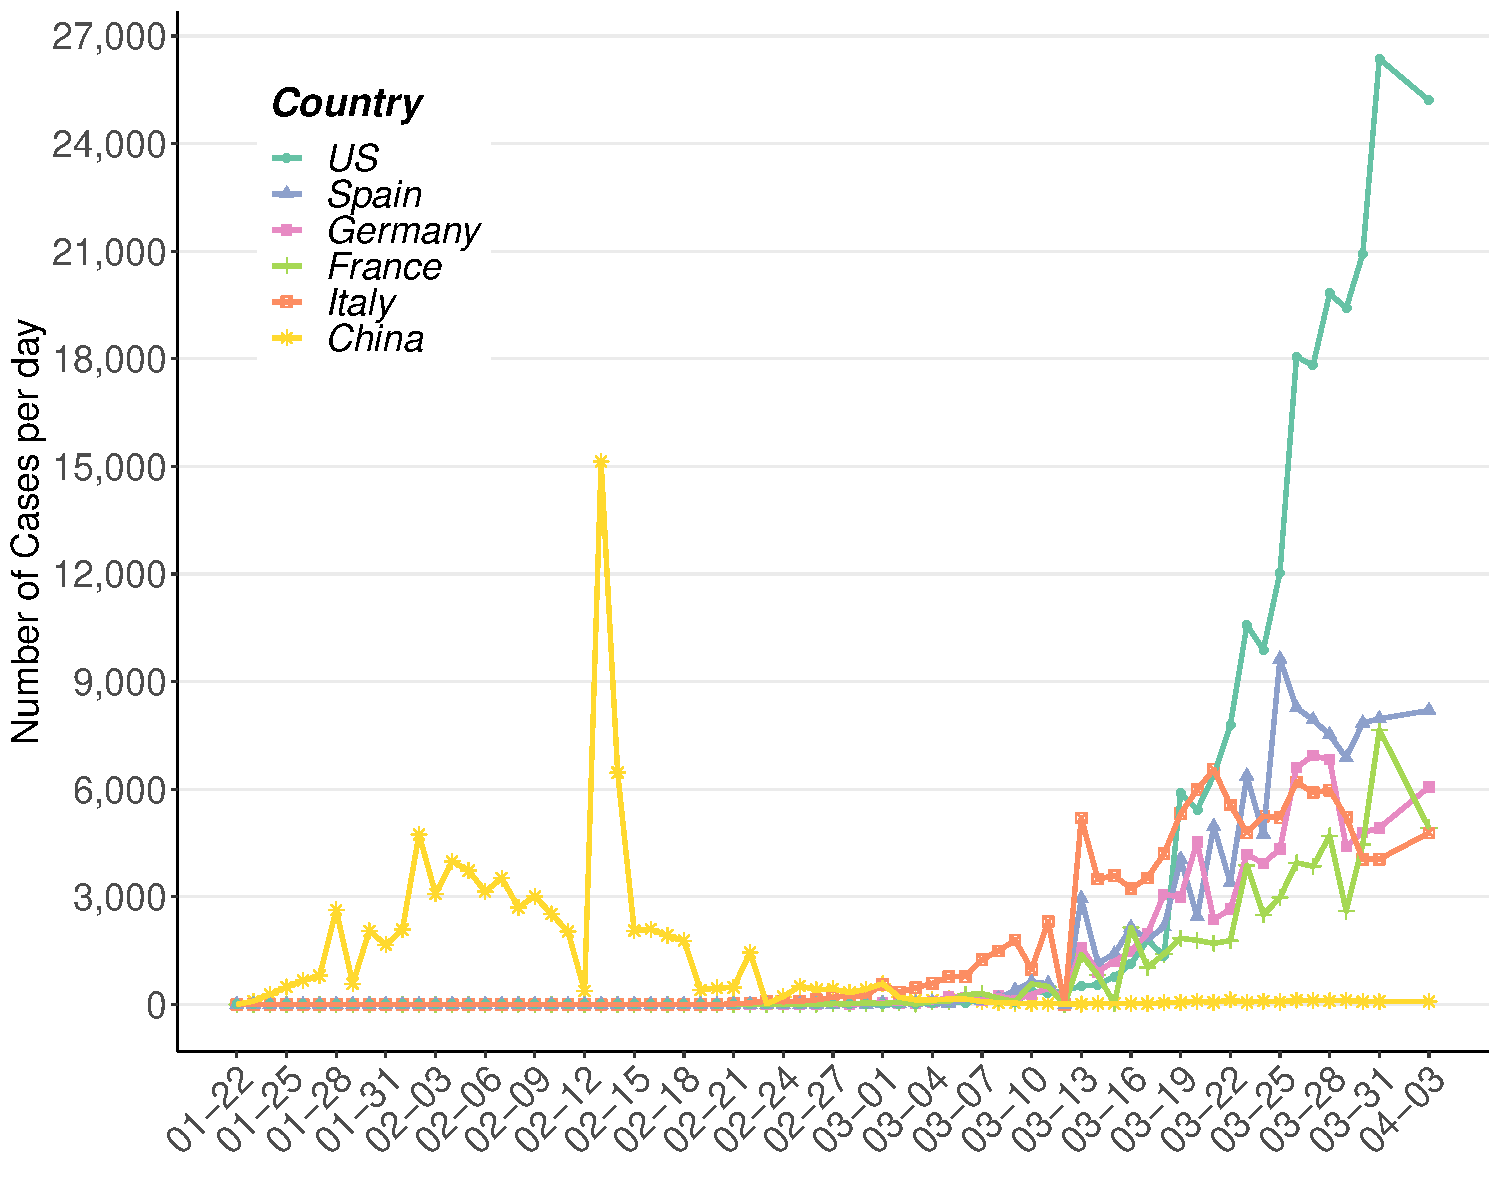
\includegraphics[]{./input/covid2.pdf}
\label{}
\end{minipage}
\quad
\begin{minipage}[b]{0.45\linewidth}
\caption{累计死亡病例国家趋势图\\(中国及其他前五位国家) }
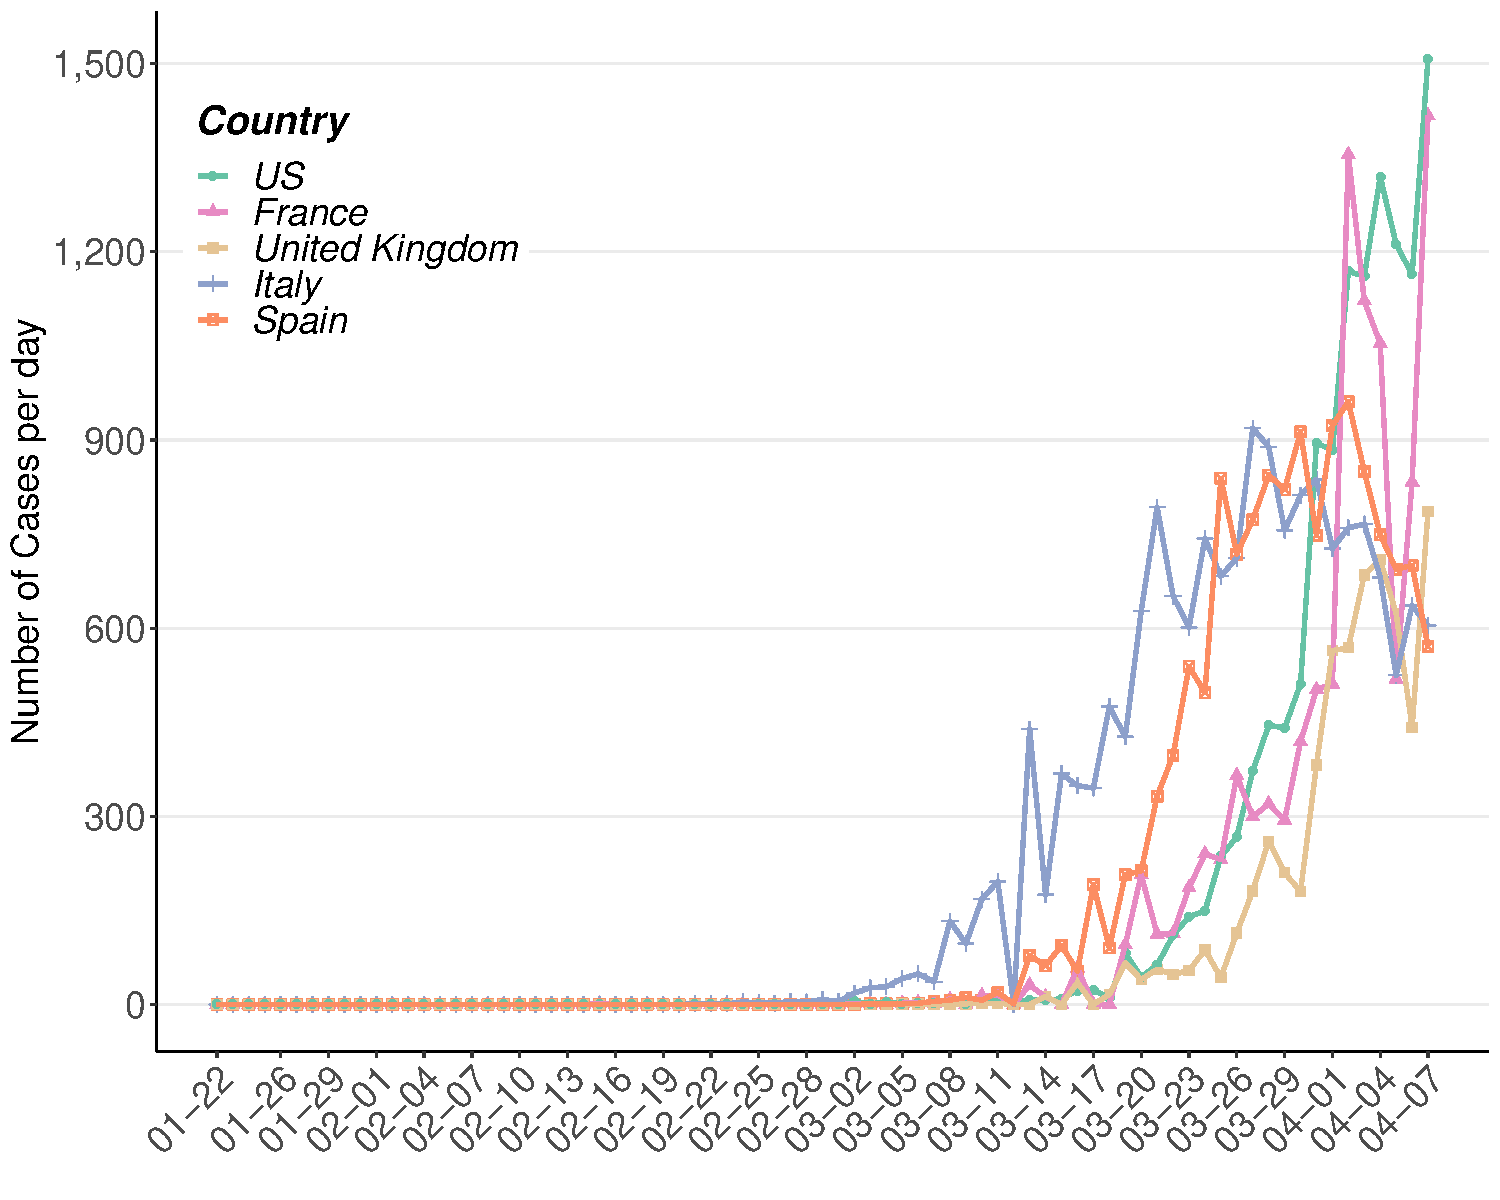
\includegraphics[]{./input/covid3.pdf}
\label{}
\end{minipage}
\end{figure}

\newpage

\hypertarget{section-3}{%
\section{\texorpdfstring{\textcolor{glaucous}{二、美国疫情}}{}}\label{section-3}}

~~截至北京时间4月3日早5:00, 美国累计确诊病例数已达到238,820例,共
5,758例死亡病例。从州疫情分布图(图4,图5)来看,确诊病例主要集中于沿海地区,对比前几日数据可见逐步向中部蔓延,有全国爆发趋势。

~~纽约州(NY)粗发病率达到475/10万人,累计确诊数占全美39\%,较昨日有所降低(41\%),日新增确诊数较昨日小幅提高,但占全美比例较昨日(44\%)有所下降,提示其他州的疫情有进一步恶化的趋势。密歇根州、加利福尼亚州累计确诊人数均已超过1万人。路易斯安纳州(LA)新增确诊病例数进一步上升,由昨日的1187人升至2697人。密歇根州(MI)、宾夕法尼亚州(PA)以及佛罗里达州(FL)新增确诊病例数均超过一千人,提示疫情在美国迅速蔓延趋势。

\begin{figure}[H] 
\caption{美国本土疫情分布图 (Map of Cumulative Confirmed COVID-19 Cases in Contiguous U.S.)} %最终文档中希望显示的图片标题
\centering
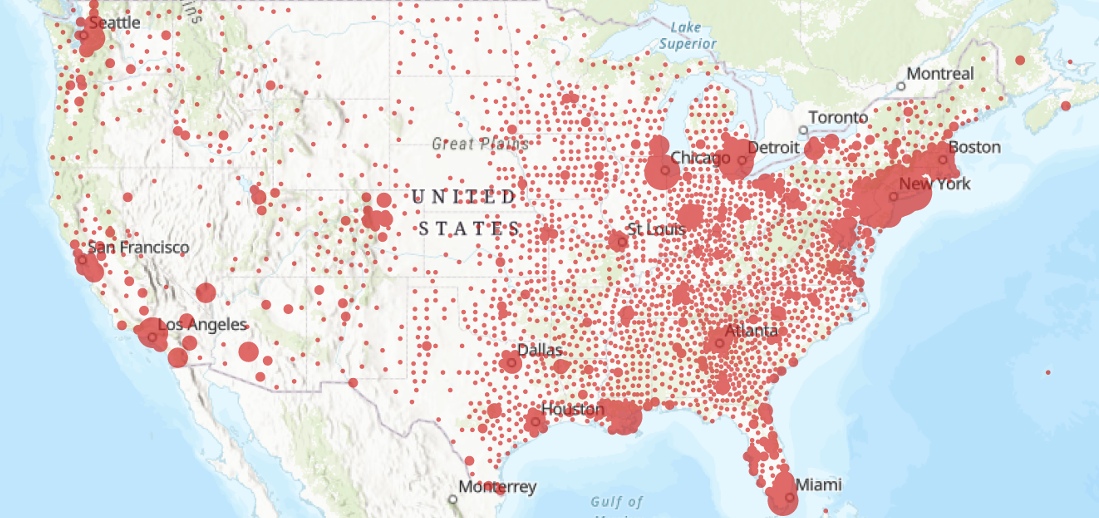
\includegraphics[]{./input/covid4.png} %插入图片,[]中设置图片大小,{}中是图片文件名
\label{} %用于文内引用的标签
\end{figure}

\begin{table}[H]
    \caption{<U+7F8E><U+56FD><U+7D2F><U+8BA1><U+786E><U+8BCA><U+524D><U+5341><U+4F4D><U+5DDE>}
      \vspace{-0.5\baselineskip}
      \centering \begin{table}[H]
\centering
\begin{tabular}{rlrrrrrr}
\toprule
  & <U+5DDE><U+540D> & <U+7D2F><U+8BA1><U+786E><U+8BCA> & <U+7C97><U+53D1><U+75C5><U+7387> & <U+9633><U+6027><U+7387>\% & <U+7D2F><U+8BA1><U+68C0><U+6D4B> & <U+65E5><U+65B0><U+589E><U+68C0><U+6D4B> & <U+68C0><U+6D4B><U+7387>\\
\midrule
\rowcolor{gray!6}   & <U+7F8E><U+56FD> US & 368,241 & 111 & 19 & 1,917,095 & 155,063 & 579\\
1 & <U+7EBD><U+7EA6><U+5DDE> NY & 131,815 & 678 & 41 & 320,811 & 18,531 & 1,649\\
\rowcolor{gray!6}  2 & <U+65B0><U+6CFD><U+897F><U+5DDE> NJ & 41,090 & 463 & 46 & 89,032 & 6,866 & 1,002\\
3 & <U+5BC6><U+6B47><U+6839><U+5DDE> MI & 17,221 & 172 & 36 & 47,251 & 1,503 & 473\\
\rowcolor{gray!6}  4 & <U+52A0><U+5229><U+798F><U+5C3C><U+4E9A><U+5DDE> CA & 16,347 & 41 & 14 & 117,431 & 898 & 297\\
5 & <U+8DEF><U+6613><U+65AF><U+5B89><U+90A3><U+5DDE> LA & 14,867 & 320 & 21 & 69,166 & 8,841 & 1,488\\
\rowcolor{gray!6}  6 & <U+9A6C><U+8428><U+8BF8><U+585E><U+5DDE> MA & 13,837 & 199 & 18 & 76,429 & 4,492 & 1,100\\
7 & <U+4F5B><U+7F57><U+91CC><U+8FBE><U+5DDE> FL & 13,629 & 63 & 11 & 123,274 & 9,870 & 574\\
\rowcolor{gray!6}  8 & <U+5BBE><U+5915><U+6CD5><U+5C3C><U+4E9A><U+5DDE> PA & 13,206 & 103 & 16 & 83,854 & 6,083 & 655\\
9 & <U+4F0A><U+5229><U+8BFA><U+4F0A><U+5DDE> IL & 12,262 & 97 & 19 & 62,942 & 3,959 & 497\\
\rowcolor{gray!6}  10 & <U+534E><U+76DB><U+987F><U+5DDE> WA & 8,384 & 110 & 9 & 91,375 & 3,457 & 1,200\\
\bottomrule
\end{tabular}
\end{table} \begin{tablenotes}
    \footnotesize
    \item <U+6CE8>: <U+68C0><U+6D4B><U+7387><U+5B9A><U+4E49>:<U+7D2F><U+8BA1><U+68C0><U+6D4B><U+4EBA><U+6570>/10<U+4E07><U+4EBA><U+3002><U+8BA1><U+7B97><U+65B9><U+5F0F>:(<U+7D2F><U+8BA1><U+68C0><U+6D4B><U+4EBA><U+6570>/<U+4EBA><U+53E3>)*10<U+4E07>
    \end{tablenotes}
    \end{table}

\newpage

\begin{figure}[H]
\centering
\begin{minipage}[b]{0.45\linewidth}
\caption{美国累计确诊前五位州趋势图}
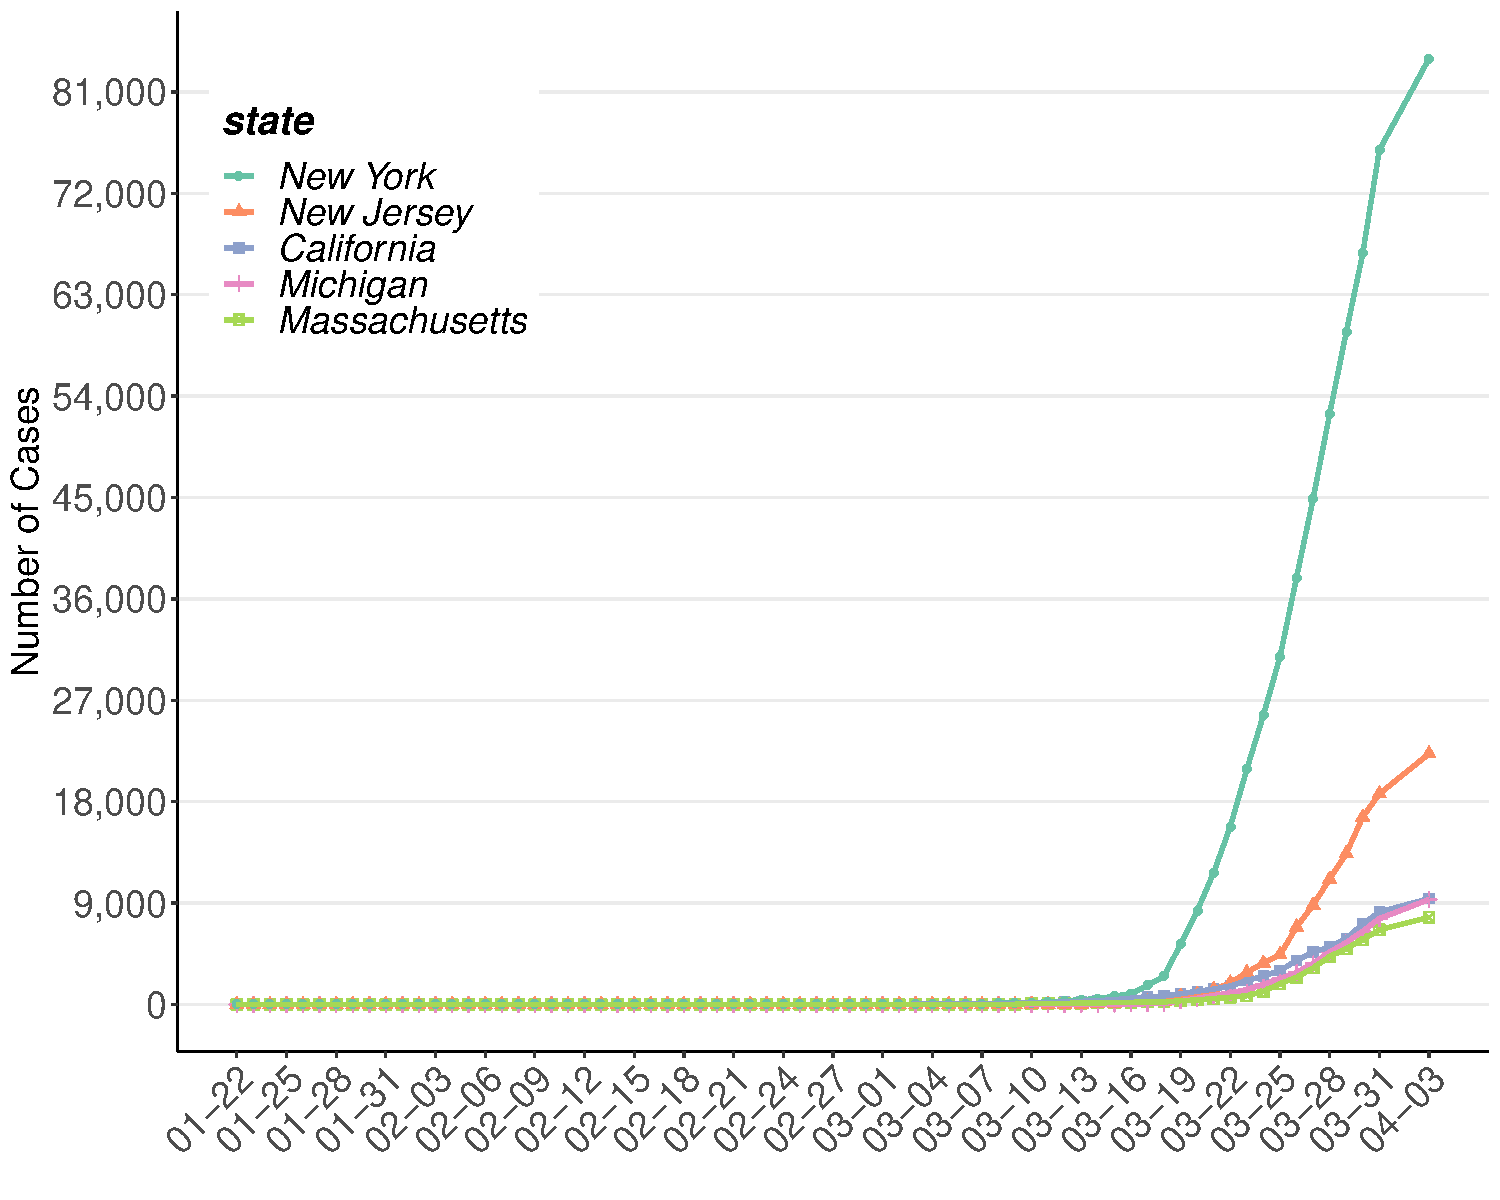
\includegraphics[]{./input/covid5.pdf}
\label{}
\end{minipage}
\quad
\begin{minipage}[b]{0.45\linewidth}
\caption{美国⽇新增确诊前五位州趋势图}
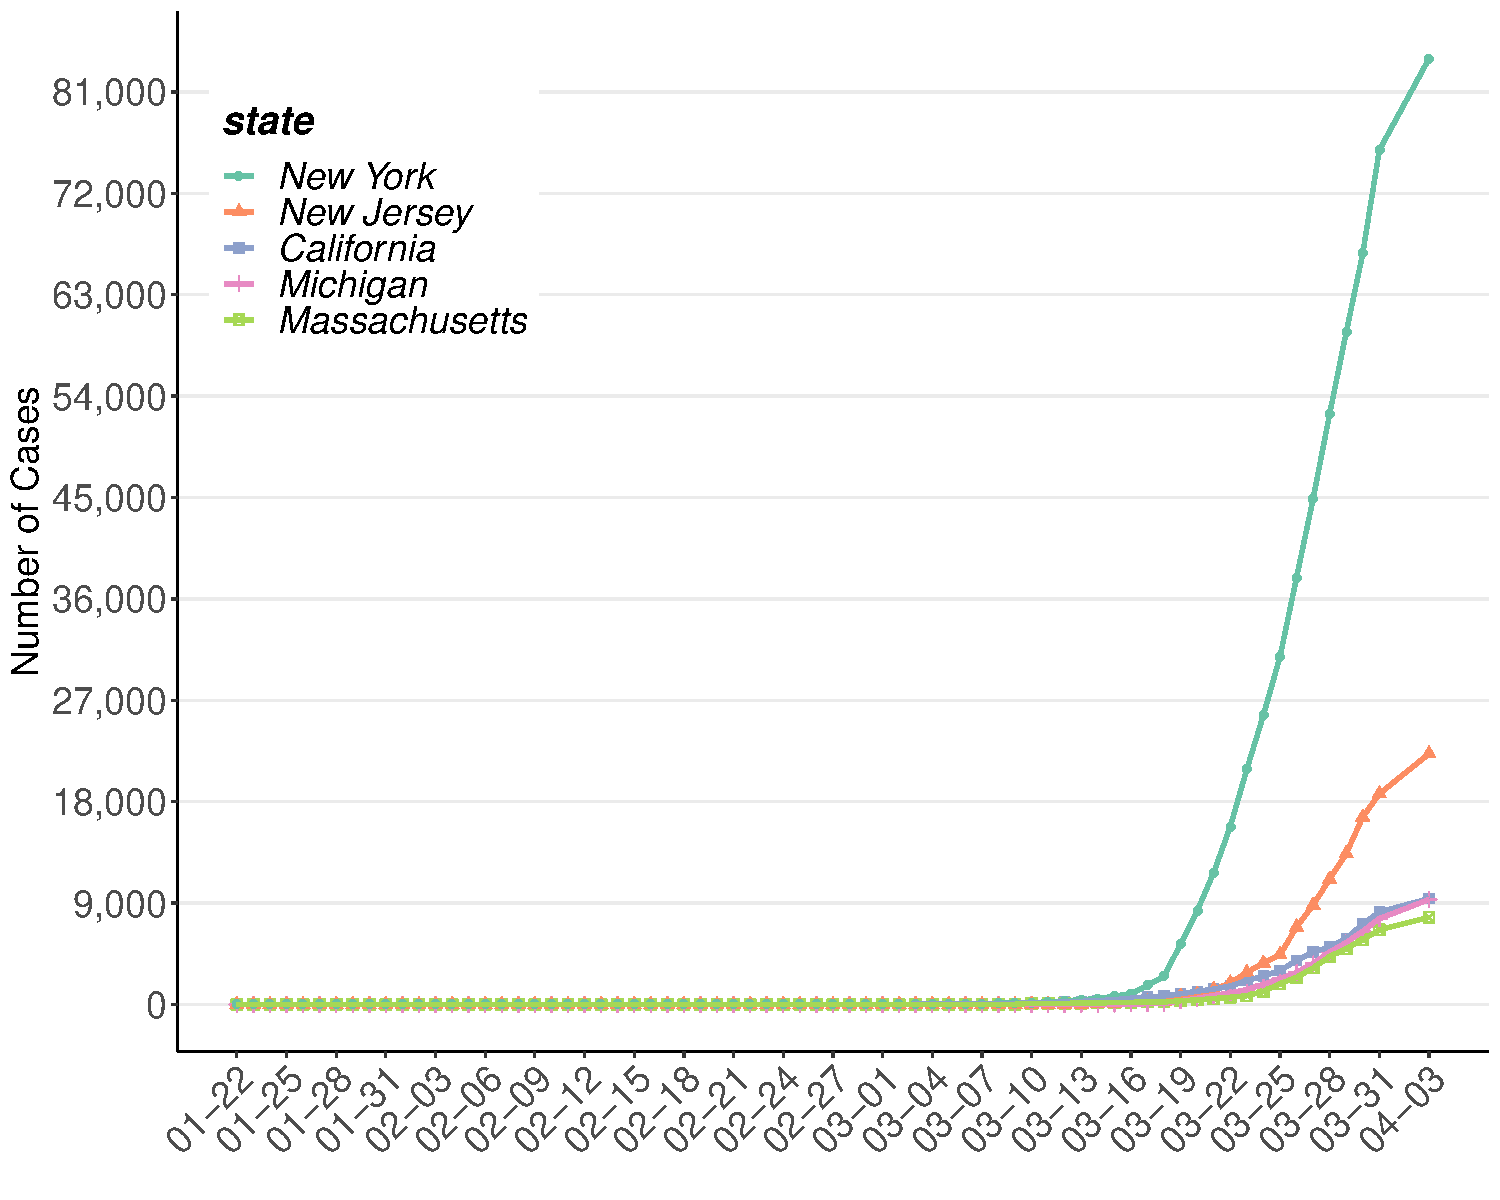
\includegraphics[]{./input/covid5.pdf}
\label{}
\end{minipage}
\end{figure}

\begin{table}
    \begin{minipage}{.4\linewidth}
    \caption{<U+786E><U+8BCA><U+524D><U+5341><U+4F4D><U+56FD><U+5BB6>}
    \vspace{-0.5\baselineskip}
      \centering
    \captionsetup{justification=centering} \begin{table}[H]
\centering
\begin{tabular}{rlrr}
\toprule
  & <U+5DDE><U+540D> & <U+5F53><U+65E5><U+65B0><U+589E> & <U+5168><U+7F8E><U+6BD4><U+7387>\\
\midrule
\rowcolor{gray!6}   & <U+7F8E><U+56FD> US & 1,627 & 100\\
1 & <U+52A0><U+5229><U+798F><U+5C3C><U+4E9A><U+5DDE> CA & 328 & 20\\
\rowcolor{gray!6}  2 & <U+4F5B><U+7F57><U+91CC><U+8FBE><U+5DDE> FL & 305 & 19\\
3 & <U+4E54><U+6CBB><U+4E9A><U+5DDE> GA & 244 & 15\\
\rowcolor{gray!6}  4 & <U+5F97><U+514B><U+8428><U+65AF><U+5DDE> TX & 111 & 7\\
5 & <U+5317><U+5361><U+7F57><U+83B1><U+7EB3><U+5DDE> NC & 92 & 6\\
\rowcolor{gray!6}  6 & <U+5BBE><U+5915><U+6CD5><U+5C3C><U+4E9A><U+5DDE> PA & 79 & 5\\
7 & <U+534E><U+76DB><U+987F><U+5DDE> WA & 73 & 4\\
\rowcolor{gray!6}  8 & <U+7231><U+8FBE><U+8377><U+5DDE> ID & 69 & 4\\
9 & <U+4FC4><U+52D2><U+5188><U+5DDE> OR & 64 & 4\\
\rowcolor{gray!6}  10 & <U+5A01><U+65AF><U+5EB7><U+661F><U+5DDE> WI & 62 & 4\\
\bottomrule
\end{tabular}
\end{table} \end{minipage}%
    \begin{minipage}{.7\linewidth}
     \caption{<U+7D2F><U+8BA1><U+6B7B><U+4EA1><U+524D><U+5341><U+4F4D><U+56FD><U+5BB6>}
     \vspace{-0.5\baselineskip}
      \centering
    \captionsetup{justification=centering} \begin{table}[H]
\centering
\begin{tabular}{rlrr}
\toprule
  & <U+5DDE><U+540D> & <U+7D2F><U+8BA1><U+6B7B><U+4EA1><U+4EBA><U+6570> & <U+75C5><U+6B7B><U+7387>\\
\midrule
\rowcolor{gray!6}   & <U+7F8E><U+56FD> US & 10,986 & 3.0\\
1 & <U+7EBD><U+7EA6><U+5DDE> NY & 4,758 & 3.6\\
\rowcolor{gray!6}  2 & <U+65B0><U+6CFD><U+897F><U+5DDE> NJ & 1,003 & 2.4\\
3 & <U+5BC6><U+6B47><U+6839><U+5DDE> MI & 727 & 4.2\\
\rowcolor{gray!6}  4 & <U+8DEF><U+6613><U+65AF><U+5B89><U+90A3><U+5DDE> LA & 512 & 3.4\\
5 & <U+52A0><U+5229><U+798F><U+5C3C><U+4E9A><U+5DDE> CA & 388 & 2.4\\
\rowcolor{gray!6}  6 & <U+534E><U+76DB><U+987F><U+5DDE> WA & 383 & 4.6\\
7 & <U+4F0A><U+5229><U+8BFA><U+4F0A><U+5DDE> IL & 308 & 2.5\\
\rowcolor{gray!6}  8 & <U+4E54><U+6CBB><U+4E9A><U+5DDE> GA & 294 & 3.9\\
9 & <U+9A6C><U+8428><U+8BF8><U+585E><U+5DDE> MA & 260 & 1.9\\
\rowcolor{gray!6}  10 & <U+4F5B><U+7F57><U+91CC><U+8FBE><U+5DDE> FL & 254 & 1.9\\
\bottomrule
\end{tabular}
\end{table} \end{minipage} 
\end{table}

~~从表6来看,全美累计阳性率前四位阳性率均为接近40\%及以上,提示有大量轻症及无症状感染者未被检出,感染人数远超报告数字,疫情严峻。全美共检测126.7万人,累计检测人数最多的三个州是纽约州(23.9万人)、佛罗里达州(7.7万人)及华盛顿州(7.5万人),其中佛罗里达州及华盛顿州阳性率均在10\%以下,提示疫情控较好。从表7全国累计死亡人数来看,各州死亡人数继续增高,病死率较昨日较为稳定。其中纽约州的累计死亡病例最多,病死率为2.6\%,略高于全国平均病死率。华盛顿州、密歇根州及路易斯安娜州的病死率也均明显高于全国平均。

~~XXXXXXX.

\newpage

%
  \noindent\fcolorbox{lavenderblush}{lavenderblush}{\makebox[\dimexpr\textwidth-2\fboxsep-2\fboxrule][l]{\textbf{~\Large 疫情观察}}}%

\hypertarget{section-4}{%
\section{\texorpdfstring{\textcolor{glaucous}{全球卫生体系最薄弱国家之一 — 非洲:塞拉利昂}}{}}\label{section-4}}

据《金融时报》报道,塞拉利昂750万人口,已有6人被确诊新冠肺炎,可塞拉利昂只有一台呼吸机。这台唯一的呼吸机在当地的一家私人医院,当地17家公立医院均无呼吸机。
造成塞拉利昂防疫形势严峻的原因有很多。主要原因由如下几点: 1.
塞拉利昂是世界上最不发达国家之一,经济发展水平落后,医疗资源匮乏。
1991-2001,该国经历了长达十年之久的内战。在2014年联合国开发计划署发布的人类发展指数排名中,塞拉利昂排名倒数第五。其首都弗里敦的面积只有整个国
家的1/200,却承受着这个全国1/5人口的压力,且失业率高达70\%。2017年全国注册医生不到200名。
2.
2塞拉利昂的公共卫生体系发展不全面。塞拉利昂曾经是埃博拉病毒的重灾区,尽管在对抗埃博拉之后政府成立了公共卫生应急处理中心,但是由于国内无法量产抗疫物资,依然需要依靠外国援助来解决相关问题。
3.
新冠疫情已经在非洲大陆快速扩散。截至4月5日,非洲已有51个国家报告出现新冠确诊病例,累计确诊人数8,736人。而两周前,非洲累计确诊人数仅为1,654
例。在两周之内,非洲确诊人数就增长了4倍。由于防疫能力和资源有限,塞拉利昂无法同时在控制本土病例的同时兼顾严防输入型病例1,使疫情防控雪上加霜。\\
我国政府长期以来支持非洲公共卫生事业的发展。早在2016年6月,中非就共同签署了《中华人民共和国商务部和非洲联盟委员会关于开展非洲疾病预防控制中心合作谅解备忘录》。2016年塞拉利昂总统欧内斯特·巴伊·科罗马访问中国时特别到访了中国疾控中心,商议中塞公共卫生技术合作相关事宜2。
目前我国国内疫情局势相对稳定,已大规模复工复产,医用防护服、医用防护口罩\面罩、测温仪、呼吸机产能已基本能满足国内需求,企业也正尽力组织扩大出口3。
在未来一段时间的抗疫物资援助和贸易上,我国相关产业可更多的将目光放在类似塞拉利昂这样的医疗资源和经济基础更加薄弱的国家。

\begin{small}{
参考文献:
1. 南财快评之全球疫情观察:从塞拉利昂看非洲防控https://k.sina.com.cn/article_1651428902_626ece2602000p2bm.html?from=news&subch=onews
2. 塞拉利昂总统访华,为何首站选择疾控中心?https://mp.weixin.qq.com/s/lf5e9PfSU7LF-3FiNoi72A 
3. 工信部:中国呼吸机产能无法满足全球疫情防控需求https://baijiahao.baidu.com/s?id=1663393284129099919&wfr=spider&for=pc}
\end{small}

\centering
\small
\begin{tabular}{ll}

主编:马晶  &  副主编:薛成海\,  仁晖 \, 何鸿恺 \\
执行责任编辑:史珂玮 \, 王冠  & 新闻组:张宁\, 张心其 \\
可视化组:霍舒同\, 张立达 & 数据分析:杜兆慧 \\
\multicolumn{2}{l}{感谢所有为日报作出贡献的志愿者:李忠锦 \, 慕帼眉\, 李祎杰}

\end{tabular}

\end{document}
